%----------------------------------------------------------------------------------------
%    PACKAGES AND THEMES
%----------------------------------------------------------------------------------------
\documentclass[aspectratio=169,xcolor=dvipsnames]{beamer}
\makeatletter
\def\input@path{{theme/}}
\makeatother
% \usetheme{CleanEasy}
\usepackage[utf8]{inputenc}
\usepackage{lmodern}
\usepackage[T1]{fontenc}
% \usepackage[brazil]{babel}
\usepackage{fix-cm}
\usepackage{amsmath}
\usepackage{mathtools}
\usepackage{listings}
\usepackage{xcolor}
\usepackage{hyperref}
\usepackage{graphicx} % Allows including images
\usepackage{booktabs} % Allows the use of \toprule, \midrule and \bottomrule in tables
\usepackage{tikz}
\usetikzlibrary{positioning, shapes, arrows, calc, decorations.pathreplacing, arrows.meta, backgrounds, patterns, overlay-beamer-styles}
\usepackage{etoolbox}
% \usepackage{animate}

%----------------------------------------------------------------------------------------
%    LAYOUT CONFIGURATION
%----------------------------------------------------------------------------------------



% Configure code listings
\lstset{
  basicstyle=\ttfamily\small,
  keywordstyle=\color{blue},
  commentstyle=\color{green!60!black},
  stringstyle=\color{red},
  showstringspaces=false,
  breaklines=true,
  frame=single,
  rulecolor=\color{black!30},
  backgroundcolor=\color{black!5},
  numbers=left,
  numberstyle=\tiny\color{black!70},
  numbersep=5pt
}

%----------------------------------------------------------------------------------------
%    TITLE PAGE
%----------------------------------------------------------------------------------------


%---------------------------------------------


\title[Nice Title]{Fancy and Elaborated Title}

\author[A. Name]{First Author\inst{1} \and  Second Author\inst{2} \and Third Author\inst{3} }

\institute[VFU]{\inst{1}%
  Faculty of Physics\\
  Very Famous University
  \and
  \inst{2}%
  Faculty of Chemistry\\
  Very Famous University 
  \and
  \inst{3}%
  Faculty of Engineering\\
  Another Very Famous University
}


\vspace{-2cm}\date{June 4, 2025}
% Define positions for logos on title page
\titlegraphic{
  \begin{tikzpicture}[remember picture, overlay]
    % 
    \node[anchor=south west, xshift=0.5cm, yshift=0cm] at (current page.south west) {
      
\includegraphics[height=1.3cm]{logos/CleanEasy-logo1.png}
    };

    % 
    \node[anchor=south west, xshift=2.5cm, yshift=0cm] at (current page.south west) {
      
\includegraphics[height=0.9cm]{logos/CleanEasy-logo2.png}
    };
    
    % 
    \node[anchor=north east, xshift=-0.8cm, yshift=-0.3cm] at (current page.north east) {
      
\includegraphics[height=1.1cm]{logos/CleanEasy-logo3.png}
    };
    
    %
    \node[anchor=north east, xshift=-2.8cm, yshift=-0.3cm] at (current page.north east) {
      
\includegraphics[height=1.4cm]{logos/CleanEasy-logo4.png}
    };
  \end{tikzpicture}
}


%----------------------------------------------------------------------------------------


\begin{document}

\begin{frame}[plain]
  \titlepage
\end{frame}

\begin{frame}[plain]{Contents}
  \tableofcontents
\end{frame}

\section{Introduction}
\begin{frame}{Introduction}
  The CleanEasy Beamer theme provides a clean, professional look for academic and business presentations.
  
  \vspace{0.3cm}
  
  Key features:
  \begin{itemize}
    \item Clean, minimalist design
    \item Carefully chosen color scheme
    \item Professional typography
    \item Flexible block environments
    \item Customizable footers and section pages
  \end{itemize}
  
  \begin{block}{About this template}
    This presentation serves as both documentation and demonstration, showing the various elements and features available in the CleanEasy theme.
  \end{block}
\end{frame}

\begin{frame}{Block environments}

  \begin{exampleblock}{Example block}
    Example blocks can be used to showcase code, examples, or case studies.
  \end{exampleblock}
  
  \begin{alertblock}{Alert block}
    Alert blocks draw attention to critical information, warnings, or caveats.
  \end{alertblock}
  
  \begin{theorem}
    In a right-angled triangle, the square of the hypotenuse equals the sum of squares of the other two sides.
  \end{theorem}
  
  \begin{definition}
    A prime number is a natural number greater than 1 that cannot be formed by multiplying two smaller natural numbers.
  \end{definition}
\end{frame}

\section{Methods}
\begin{frame}{Lists and Numbering}
  \begin{columns}
    \begin{column}{0.48\textwidth}
      Bulleted list:
      \begin{itemize}
        \item First level item
        \begin{itemize}
          \item Second level item
          \item Another second level
          \begin{itemize}
            \item Third level item
          \end{itemize}
        \end{itemize}
        \item Another first level item
      \end{itemize}
    \end{column}
    \begin{column}{0.48\textwidth}
      Numbered list:
      \begin{enumerate}
        \item First step
        \begin{enumerate}
          \item Substep one
          \item Substep two
        \end{enumerate}
        \item Second step
        \item Third step
      \end{enumerate}
    \end{column}
  \end{columns}
\end{frame}

\begin{frame}{Tables}
  \begin{table}
    \centering
    \caption{Sample table with booktabs style}
    \begin{tabular}{lcr}
      \toprule
      \textbf{Header 1} & \textbf{Header 2} & \textbf{Header 3} \\
      \midrule
      Row 1, Col 1 & Row 1, Col 2 & 123.45 \\
      Row 2, Col 1 & Row 2, Col 2 & 67.89 \\
      Row 3, Col 1 & Row 3, Col 2 & 456.78 \\
      \bottomrule
    \end{tabular}
  \end{table}
  
  \vspace{0.5cm}
  
  \begin{block}{Table styling}
    The CleanEasy theme works well with the booktabs package for professional-looking tables. 
    Simple color alterations make tables more readable without being distracting.
  \end{block}
\end{frame}

\begin{frame}{Mathematical Equations}
  The CleanEasy theme includes proper mathematical typesetting:
  
  \begin{align}
    E &= mc^2 \\
    F &= G\frac{m_1 m_2}{r^2}
  \end{align}
  
  Maxwell's equations in differential form:
  \begin{align}
    \nabla \cdot \vec{E} &= \frac{\rho}{\varepsilon_0} \\
    \nabla \cdot \vec{B} &= 0 \\
    \nabla \times \vec{E} &= -\frac{\partial \vec{B}}{\partial t} \\
    \nabla \times \vec{B} &= \mu_0 \vec{J} + \mu_0\varepsilon_0\frac{\partial \vec{E}}{\partial t}
  \end{align}
  
  Inline equations like $E = mc^2$ are also properly rendered.
\end{frame}

\begin{frame}[fragile]{Code Listings}
  \begin{lstlisting}[language=Python]
# A simple Python function
def fibonacci(n):
    """Return the nth Fibonacci number"""
    if n <= 0:
        return 0
    elif n == 1:
        return 1
    else:
        a, b = 0, 1
        for _ in range(2, n + 1):
            a, b = b, a + b
        return b
  
# Calculate the 10th Fibonacci number
result = fibonacci(10)
print(f"The 10th Fibonacci number is {result}")
  \end{lstlisting}
\end{frame}

\begin{frame}{Figures and Graphics}
  \begin{columns}
    \begin{column}{0.48\textwidth}
      \centering
      \begin{figure}
        \centering
        % Replace with actual image path
        % \includegraphics[width=\textwidth]{figures/sample_image.png}
        \tikz \fill[blue!30] (0,0) rectangle (3,2);
        \caption{Sample placeholder image}
      \end{figure}
    \end{column}
    \begin{column}{0.48\textwidth}
      \centering
      \begin{figure}          
      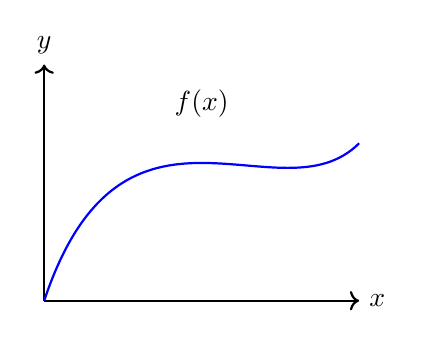
\begin{tikzpicture}
        % Simple TikZ diagram
        \draw[thick, ->] (0,0) -- (4,0) node[right] {$x$};
        \draw[thick, ->] (0,0) -- (0,3) node[above] {$y$};
        \draw[blue, thick] (0,0) .. controls (1,3) and (3,1) .. (4,2);
        \node at (2,2.5) {$f(x)$};
      \end{tikzpicture}
      \caption{Simple TikZ diagram}
       \label{fig:enter-label}
      \end{figure}
    \end{column}
  \end{columns}
\end{frame}

\section{Results}
\begin{frame}{Overlays and Animations}
  Beamer supports step-by-step revelations:
  
  \begin{itemize}
    \item<1-> First point appears on slide 1
    \item<2-> Second point appears on slide 2
    \item<3-> Third point appears on slide 3
  \end{itemize}
  
  \pause
  
  This text appears after a pause.
  
  \onslide<4->{
    And this content appears on slide 4.
  }
  
  \begin{block}<5->{Delayed Block}
    This entire block appears only on slide 5.
  \end{block}
\end{frame}

\begin{frame}{Citations and References}
  CleanEasy works well with bibliographies and citations:
  
  \begin{block}{Sample citation}
    % According to Einstein \cite{einstein1905}, space and time are relative.
  \end{block}
  
  \begin{exampleblock}{Bibliography management}
    The theme is compatible with BibTeX, BibLaTeX, and other bibliography management tools.
  \end{exampleblock}
  
  % Sample bibliography entries (not functional without .bib file)
  % \begin{thebibliography}{9}
  % \bibitem{einstein1905}
  %   Albert Einstein.
  %   \emph{On the Electrodynamics of Moving Bodies}.
  %   Annalen der Physik, 1905.
  % \end{thebibliography}
\end{frame}

\begin{frame}{Custom TikZ Graphics}

  \begin{figure}
      \centering
      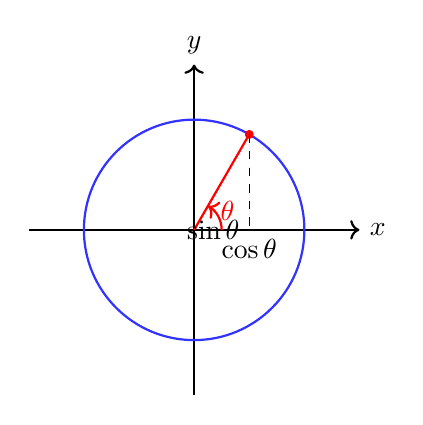
\begin{tikzpicture}[scale=0.7]
        % Coordinate axes
        \draw[thick, ->] (-3,0) -- (3,0) node[right] {$x$};
        \draw[thick, ->] (0,-3) -- (0,3) node[above] {$y$};
        
        % Unit circle
        \draw[blue!80, thick] (0,0) circle (2);
        
        % Angle and point on circle
        \filldraw[red] (60:2) circle (2pt);
        \draw[red, thick] (0,0) -- (60:2);
        \draw[red, thick, ->] (0.5,0) arc (0:60:0.5);
        \node[red] at (30:0.7) {$\theta$};
        
        % Coordinates
        \draw[dashed] (60:2) -- (60:2 |- 0,0) node[below] {$\cos\theta$};
        \draw[dashed] (60:2) -- (0,0 -| 60:2) node[left] {$\sin\theta$};
      \end{tikzpicture}
      \caption{The unit circle with trigonometric functions}
      \label{fig:exampleTikz}
  \end{figure}
\end{frame}

\section{Conclusions}
\begin{frame}{Theme Customization}
  The CleanEasy theme can be easily customized:
  
  \begin{itemize}
    \item Edit \texttt{beamercolorthemeCleanEasy.sty} to change colors
    \item Modify \texttt{beamerfontthemeCleanEasy.sty} for different fonts
    \item Adjust \texttt{beamerinnerthemeCleanEasy.sty} for layout changes
    \item Update \texttt{configs.tex} for footer and section page customization
  \end{itemize}
  
  \begin{alertblock}{Important Note}
    Always maintain consistent design elements throughout your presentation for a professional look.
  \end{alertblock}
\end{frame}

\begin{frame}{Final Thoughts}
  \begin{block}{Benefits of CleanEasy}
    \begin{itemize}
      \item Professional appearance suitable for academic and business contexts
      \item Careful attention to typography and spacing
      \item High readability with suitable contrast ratios
      \item Flexible design that works with different content types
    \end{itemize}
  \end{block}
  
  \vspace{0.5cm}
  
  \begin{center}
    \large{The CleanEasy theme is designed to let your content shine without distractions}
  \end{center}
\end{frame}

\begin{frame}[plain]
  \centering
  \Huge \textbf{Thank you!}
  
  \vspace{1cm}
  \normalsize
  \href{mailto:your@email.com}{your@email.com}
  
  \vspace{0.5cm}
  \small
  \texttt{https://someurl.com}
\end{frame}

% Sample bibliography (not shown in presentation, just for reference)
\begin{frame}{References}
  \begin{thebibliography}{9}
    \bibitem{einstein1905}
      Albert Einstein.
      \emph{On the Electrodynamics of Moving Bodies}.
      Annalen der Physik, 1905.
    
    \bibitem{beamer}
      Till Tantau.
      \emph{The Beamer Class}.
      \url{https://ctan.org/pkg/beamer}
  \end{thebibliography}
\end{frame}

% \begin{frame}{References}
%   \bibliography{reference.bib}
%   \bibliographystyle{apalike}
% \end{frame}

\end{document}